\documentclass[final, slidestop]{beamer}

\title{Generating variant descriptions based on sequence comparison}
\author{Jeroen F.J. Laros, Martijn Vermaat, Johan T. den Dunnen,
  Peter E.M. Taschner}
\institute{Center for Human and Clinical Genetics, Leiden University Medical
  Center, Leiden, The Netherlands}
\providecommand{\centerLogo}{
  \includegraphics[height = 3cm]{gen2phen_logo}
}
\providecommand{\rightLogo}{
  \includegraphics[height = 3cm]{nbic_logo}
}
\providecommand{\colOneWidth}{0.48}
\providecommand{\colTwoWidth}{0.48}

\usetheme{lumc}

\begin{document}

\begin{frame}{}
  \begin{myPoster}
    \colorBlock{Background}{Introduction}{1}{
      Unambiguous and correct sequence variant descriptions are of utmost
      importance for DNA diagnostics. Descriptions can be checked and corrected
      with the {\em Mutalyzer sequence variation nomenclature checker}
      (Fig.~\ref{figure:namecheck}) (\color{red}\bt{https://mutalyzer.nl/}\color{LUMCBlue})
      following the Human Genome Variation Society (HGVS) sequence variant
      nomenclature recommendations~\cite{HGVS}.

      \vspace{1cm}

      Initial construction of variant descriptions, however, requires comparison
      of the reference sequence and the variant sequence and basic knowledge of
      the HGVS recommendations. With the arrival of long read sequencers (e.g.
      PacBio) and the rise of sophisticated variant callers, the chance of
      finding a complex variant increases and so does the need to describe these
      variants.

      \vspace{1cm}

      \begin{figure}
        {
          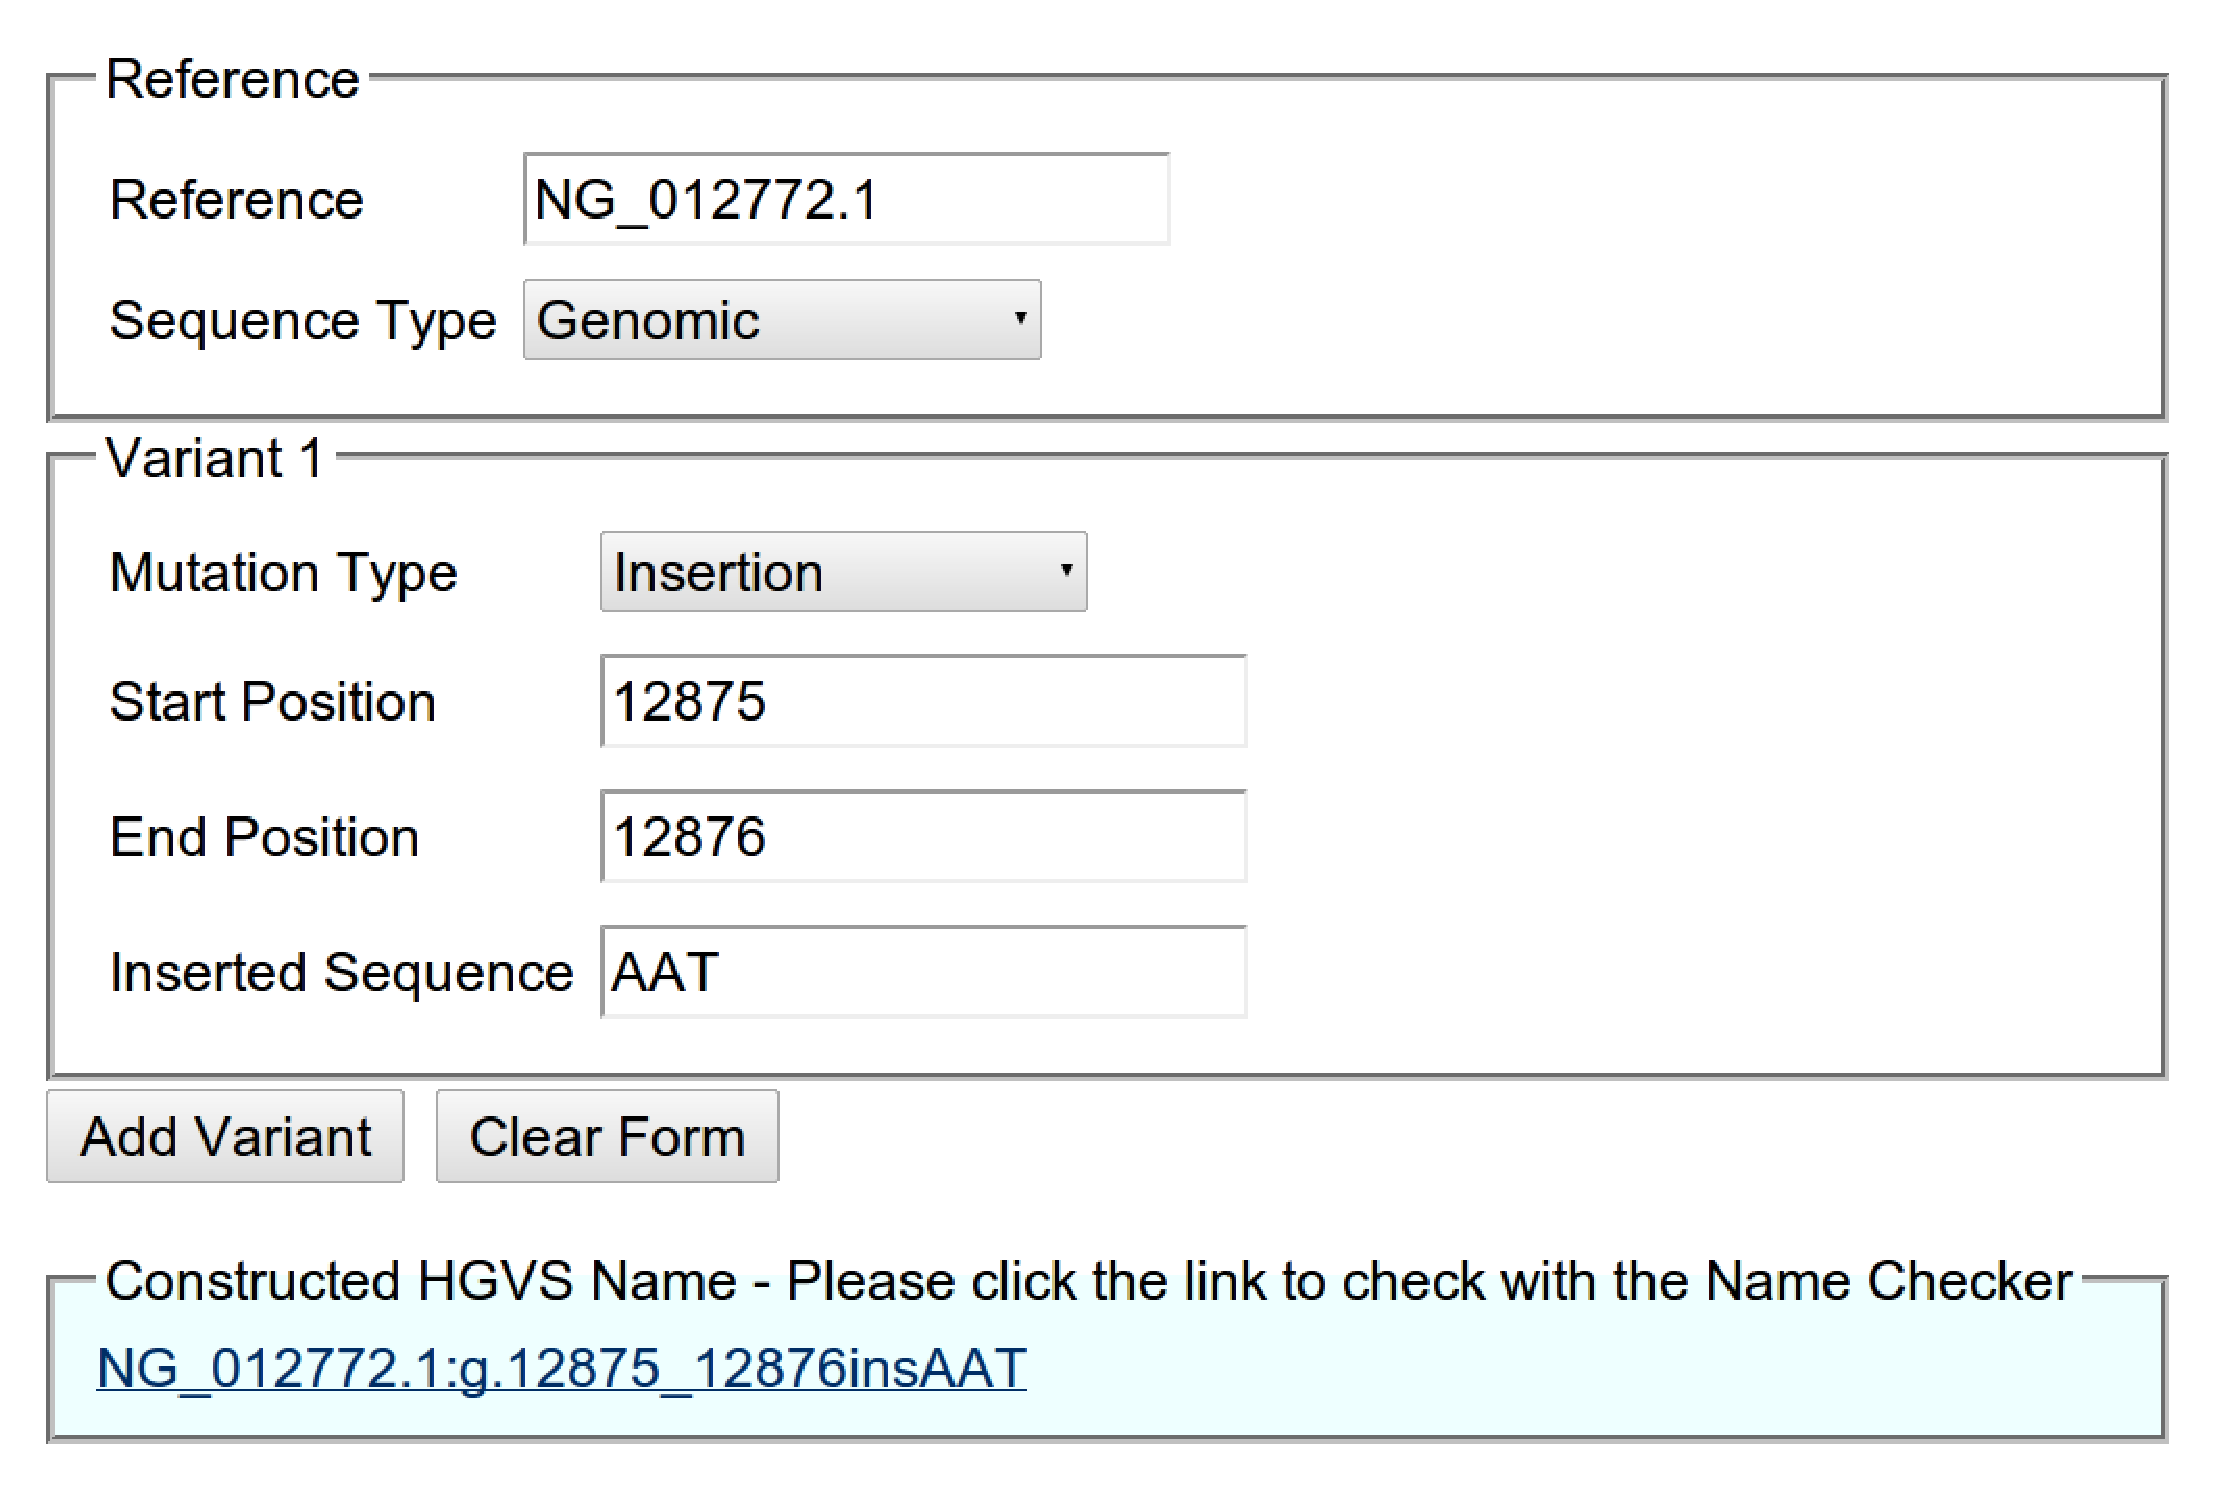
\includegraphics[width = 0.8\textwidth, height = 19cm]{mutalyzerNameGenerator}
        }
        \caption{Name Generator describing an insertion on a genomic reference
          sequence}
        \label{figure:namegenerator}
      \end{figure}

      \vspace{1cm}

      To aid in the construction of a variant description, Mutalyzer includes
      the Name Generator (Fig.~\ref{figure:namegenerator}), alleviating the
      need for knowledge of the HGVS recommendations. However, comparison of
      reference and variant sequences still has to be done by the user and can
      be a complex task.
    }
    \colorBlock{SalmonBg}{Description Extraction}{1}{
      The new Description Extractor can be used to automatically construct
      variant descriptions according to the HGVS recommendations by sequence
      comparison. The algorithm closely follows the human approach to
      describe a variant. It will first find the ``area of change'' and then
      finds the largest overlap between the original area and the area in the
      variant sequence. This process is repeated until  the smallest
      description is found. This not only helps clinicians to generate the
      correct description, but its implementation also allows automation of
      the description process.

      \vspace{1cm}

      As an example, consider the following two DNA sequences:

      \vspace{1cm}

      \texttt{~~~\textcolor{blue}{A}\textcolor{red}{T}\textcolor{orange}{G}\textcolor{blue}{A}\textcolor{red}{T}~~\textcolor{orange}{G}\textcolor{blue}{A}\textcolor{red}{T}\textcolor{green}{C}\textcolor{blue}{A}\textcolor{orange}{G}\textcolor{blue}{A}\textcolor{red}{T}\textcolor{blue}{A}\textcolor{green}{C}\textcolor{blue}{A}\textcolor{orange}{G}\textcolor{red}{T}\textcolor{orange}{G}\textcolor{red}{T}\textcolor{orange}{G}\textcolor{blue}{A}\textcolor{red}{T}\textcolor{blue}{A}\textcolor{green}{C}\textcolor{blue}{A}\textcolor{orange}{G}\textcolor{orange}{G}\textcolor{red}{T}\textcolor{blue}{A}\textcolor{orange}{G}\textcolor{red}{T}\textcolor{red}{T}\textcolor{blue}{A}\textcolor{orange}{G}~\textcolor{blue}{A}\textcolor{green}{C}\textcolor{blue}{A}\textcolor{blue}{A}~~~}reference\\
      \texttt{~~~|||||~~|||||||||||~||||||||~|||||||||~||||}\\
      \texttt{~~~\textcolor{blue}{A}\textcolor{red}{T}\textcolor{orange}{G}\textcolor{blue}{A}\textcolor{red}{T}\textcolor{red}{T}\textcolor{red}{T}\textcolor{orange}{G}\textcolor{blue}{A}\textcolor{red}{T}\textcolor{green}{C}\textcolor{blue}{A}\textcolor{orange}{G}\textcolor{blue}{A}\textcolor{red}{T}\textcolor{blue}{A}\textcolor{green}{C}\textcolor{blue}{A}~\textcolor{red}{T}\textcolor{orange}{G}\textcolor{red}{T}\textcolor{orange}{G}\textcolor{blue}{A}\textcolor{red}{T}\textcolor{blue}{A}\textcolor{green}{C}\textcolor{green}{C}\textcolor{orange}{G}\textcolor{orange}{G}\textcolor{red}{T}\textcolor{blue}{A}\textcolor{orange}{G}\textcolor{red}{T}\textcolor{red}{T}\textcolor{blue}{A}\textcolor{orange}{G}\textcolor{orange}{G}\textcolor{blue}{A}\textcolor{green}{C}\textcolor{blue}{A}\textcolor{blue}{A}~~~}variant

      \vspace{1cm}

      By comparing the sequences, the following HGVS description of the variant
      sequence will be extracted: \texttt{g.[5\_6insTT;17del;26A>C;35dup]}

      \vspace{1cm}

      \begin{table}
        \caption{Overview of the raw variants as provided by the Description
          Extractor}
        \colorbox{white}{
        {\small
          \begin{tabular}{l|l|l|l|l|l|l}
            Start & End & Type  & Deleted    & Inserted    & Shift & Description \\
            \hline
            5     & 6   & ins   &            & \texttt{TT} & 1     & \texttt{5\_6insTT} \\
            17    & 0   & del   &            &             & 0     & \texttt{17del} \\
            26    & 0   & subst & \texttt{A} & \texttt{C}  & 0     & \texttt{26A>C} \\
            35    & 0   & dup   &            &             & 1     & \texttt{35dup} \\
          \end{tabular}
          }
        }
      \end{table}
    }
    \colorBlock{YellowBg}{Acknowledgements}{1}{
      {\small
        Funded by the European Community's Seventh Framework Programme
        (FP7/2007-2013) under grant agreement no. 200754 - the GEN2PHEN project.
      }

    }
    \nextColumn
    \colorBlock{WhiteBg}{Conclusions}{1}{
      With this proof-of-concept we have shown that it is feasible to
      automatically generate correct variant descriptions following the HGVS
      recommendations based on a comparison of the original sequence and the
      observed sequence. The implementation relieves the user from the often
      complex task of manually creating a description and guarantees
      conformity to HGVS.

      \vspace{1cm}

      As future work we plan to implement description extraction from reference
      sequences either identified by accession number or manually uploaded.
      This will enable, for example, easy construction of descriptions for the
      difference between different versions of reference sequence, either
      genomic or transcript.
    }
    \colorBlock{BlueBg}{Name Checking}{1}{
      \begin{figure}
        {
          \includegraphics[width = 0.95\textwidth, height = 57cm]{mutalyzerNameCheck}
        }
        \caption{Name Checker results using the CDKN2A LRG reference
          sequence~\cite{LRG}}
        \label{figure:namecheck}
      \end{figure}
    }
    %\colorBlock{GreenBg}{Mutalyzer Interfaces (a Selection)}{1}{
    %  \begin{tabular}{l@{\ \ --\ \ }p{25cm}}
    %    Name Checker       & Syntactic and semantic checks.$^*$
    %                           (Fig.~\ref{figure:namecheck}) \\
    %    %Syntax Checker     & Syntactic checks only.$^*$ \\
    %    Position Converter & Convert chromosomal positions to gene-centered
    %                           notation (no semantic check).$^*$ \\
    %    %SNP Converter      & Convert a dbSNP rsId to HGVS notation.$^*$ \\
    %    Name Generator     & Contruct a HGVS notation. \\
    %    Description Extractor & Extract HGVS notation from sequences. \\
    %    %GenBank Uploader   & Upload custom GenBank files. \\
    %    Webservices        & Programmatic (SOAP) interface. \\
    %  \end{tabular}
    %  \bigskip
    %
    %  $^*$ {\small Also available as a batch interface.}
    %}
    \colorBlock{Background}{References}{1}{
      {\small
        \bibliography{$HOME/projects/bibliography}{}
      }
    }
  \end{myPoster}
\end{frame}
\end{document}
